\chapter{Обзор} \label{chapt_1}
\section{Краткий обзор по истории открытия гелия и методам его выделения} \label{section_1_1}

Гелий -- второй элемент в таблице Менделева, самый распространённый  изотоп $^4$He которого имеет среднюю атомную массу  $4,0026$~а.е.м., был обнаружен в 1968 году независимо учёными Жансеном и Локьером в спектральными методами при исследовании солнечной короны. В 1871 году Кельвин предложил назвать обнаруженное вещество <<гелий>>.
В 1895 году Рамзай при исследовании газа, выделенного из минерала клевеита, обнаружил присутствие гелия на Земле. Было установлено, что неопознанная линия спектра $D_3$, отвечавшая новому элементу, имела длину волны $5874,9$~\AA \cite{Fastovskii}.

Гелий относится к группе <<инертных>> газов. Особые свойства гелия: легкость (легче только водород H$_2$); абсолютная инертность; низкая адсорбционная способность; низкая растворимость в пластовых водах; высокая диффузионная способность и проницаемость, вызванная малым диаметром атомов ($2,7$~\AA). Стоит также отметить сверхтекучесть гелия (He-II) ниже температуру кипения $2,186$~К \cite{Yakuceni_Helium}.

Гелий имеет огромную ценность из-за своих уникальных свойств. 
Основные области применения гелия \cite{Yakuceni_Helium, Yakuceni_USA, Kryukov, Dolgushev}:
\begin{itemize}
\item сверхпроводимость (включая МРТ) -- 29~\%;
\item воздухоплавание  -- 16~\%;
\item сварка и резка металлов -- 12~\%;
\item оптико-волокно -- 7~\%;
\item аналитические цели  -- 6~\%;
\item атомная энергетика  -- 6~\%;
\item детектирование микротечей  -- 6~\%;
\item полупроводники  -- 5~\%;
\item ракетная техника  -- 4~\%;
\item выплавка металлов  -- 3~\%;
\item дыхательные смеси  -- 2~\%;
\item другие  -- 4~\%.	
\end{itemize}

Устойчивый рост годового потребления гелия составляет примерно $5$~\% в год \cite{Yakuceni_Helium}. 

После использования гелий в следствие своей лёгкости и <<текучести>>  улетучивается в атмосферу, а его утилизация является крайне трудоёмкой. Гелий является невозобновляемым ресурсом, поэтому необходимы эффективные способы выделения и хранения гелия из имеющихся ресурсов этого газа. Вопросы добычи и сохранения запасов этого газа решаются на уровне государств, обладающих этим ресурсом. Обширный обзор по на эту тему представлен в \cite{Kontorovich}.




Гелий (в основном $^4$He) в земной атмосфере (земной гелий) -- продукт $\alpha$-распада тяжелых радиоктивных элементов  (U, Th, Ac). Скорость образования гелия мала --- за один год $1$~т урана, связанного минералами, выделяет около $0,12$~см$^3$ гелия. Далее он остаётся в земной коре (в природном газе) либо рассеивается из атмосферы в космос. Содержание другого стабильного изотопа $^3$He крайне мало как в воздухе, так и в природном газе. Соотношения содержания  $^3$He/$^4$He составляет $1,1\cdot 10^{-6}$ для воздуха и $1,4\cdot 10^{-7}$ для природного газа \cite{Fastovskii}. Низкая скорость образования гелия объясняет низкое содержание гелия в природном газе и атмосфере.

В работе  \cite{Simonenko} автор обосновывает вариант извлечения гелия из воздуха на основе криогенного метода. На сегодняшний день на Земле гелий добывают в основном из природного газа, т.к. содержание гелия в атмосфере ничтожно мало, и извлечение гелия из атмосферы требует больших энергетических затрат рис.~\ref{pic:helium_cryogen_energy} (не считая сложности и капиталоемкости оборудования и его обслуживания).

\begin{figure}[ht] 
	\centering
	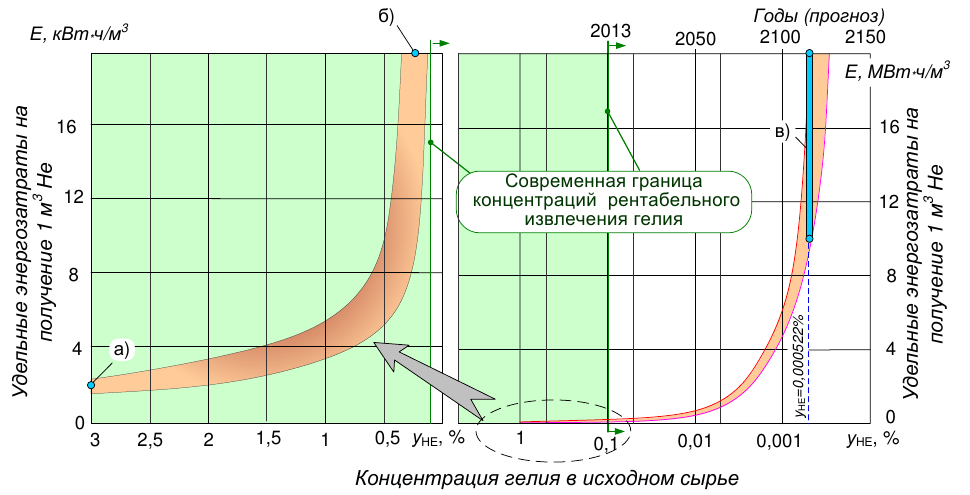
\includegraphics [width=0.9\textwidth] {part_1/helium_cryogen_energy}
	\caption{Расход энергии на извлечение гелия криогенными методами в зависимости от состава исходного сырья. Вариант в) описывает энергозатраты при добыче гелия из воздуха \cite{Simonenko}.}
	\label{pic:helium_cryogen_energy}
\end{figure}


 Месторождения природного газа по содержанию гелия делятся на несколько основных типов (Таблица \ref{tbl:He_deposit_classification}). Содержание гелия в месторождении коррелирует с возрастом продуктивных отложений \cite{Yakuceni_Material_Base}.  

\begin{table} [htbp]
	\centering
	\changecaptionwidth\captionwidth{15cm}
	\caption{Классификация природных газов по гелиеносности \cite{Yakuceni_Material_Base}}\label{tbl:He_deposit_classification}%
	\begin{tabular}{|p{5cm}||p{5cm}|p{3cm}|}
		\hline
		Преобладающие интервалы концентрации гелия, \%   & \centering Гелиесодержание в газах & \centering  $^3$He/$^4$He  \cr
		\hline
		\centering $<0,005$ & \centering  Весьма низкое  &\centering $10^{-7}$--$10^{-6}$  \cr
		\centering $0,005$-$0,009$ &\centering Низкое  &\centering $10^{-7}$--$10^{-6}$  \cr
		\centering $0,010$-$0,049$ &\centering Пониженное  &\centering $10^{-7}$  \cr		
		\centering $0,050$-$0,099$ &\centering Повышенное  &\centering $10^{-8}$  \cr		
		\centering $0,100$-$1,000$ &\centering Высокое  &\centering $10^{-8}$  \cr		
		\centering $>1,000$ &\centering Очень высокое  &\centering $10^{-8}$--$10^{-6}$ \cr		
		\hline
	\end{tabular}
\end{table}


Достаточно обширное описание сырьевой базы гелия содержится в литературе  \cite{Yakuceni_Material_Base, Kryukov}. Нужно сказать, что основная добыча гелия ведётся в США ($70$~\% от мировой), а  выделения гелия из природного газа становится  целесообразным при его содержании в смеси больше либо равном $0,1$~\%.

Месторождения газа в Восточной Сибири располагают значительными гелиеносными ресурсами углеводородов и являются идеальной базой для создания газоперерабатывающего, гелиевого и газохимического кластера для получения продукции с высокой добавленной стоимостью и создания необходимых и достаточных условий для динамичного экономического и социального развития территорий Сибири и Дальнего Востока. Подготовленные к промышленному освоению запасы природного газа Собинского, Ковыктинского и Чаяндинского месторождений составляют около $3$~трлн.~н.~м$^3$ (с гелиесодержанием от $0,2$~\% до $0,6$~\%). Прогнозные оценки освоения этих и других месторождений показывают, что Россия в ближайшем будущем может стать одним из крупнейших производителей и поставщиков гелия на внутренний и мировой рынок и одновременно удовлетворить потребности стран Юго-Восточной Азии и Тихоокеанского региона в природном газе.




Подготовка и комплексная переработка гелиеносного природного газа с целью выделения гелия, других ценных компонентов, и последующей доставки природного газа по газотранспортным сетям от месторождений к потребителям является актуальной научной и технологической задачей. Решение этой задачи и строительство газотранспортной системы <<Сила Сибири>>, объединяющей Иркутский и Якутский центры газодобычи, станет в конечном итоге важным шагом в создании единой системы газоснабжения России.

К настоящему времени для разделения газов используется три основных метода: криогенный, мембранный и адсорбционный.



\subsection{Криогенный метод извлечения гелия из природного газа} \label{section_1_1_1}

В настоящее время в промышленном масштабе гелий извлекают из природного газа с помощью криогенной технологии, физическую основу которой составляет конденсация углеводородных фракций, являющихся основными компонентами природного газа \cite{Barron}.   В результате выделение небольших объемов гелия из природного газа требует высоких энергетических и капитальных  затрат \cite{Andreev, Simonenko}. Так по ссылке \cite{LenNIIHimMash} указано, что ориентировочные энергозатраты на выделение гелия из газов, содержащих $0,02$, $0,05$, $0,35$~\% гелия, составляют $250$, $100$ и $18$~кВт$\cdot$ч/м$^3$ соответственно, что коррелирует с рис. \ref{pic:helium_cryogen_energy}.

ОАО <<НПО «Гелиймаш>> было разработано и выпущено подавляющее большинство криогенных гелиевых установок, работающих в России и странах ближнего зарубежья. Всего, начиная с первого гелиевого ожижителя, выпущенного в 60-е годы ХХ века, предприятием было поставлено около ста криогенных гелиевых установок различной производительности для научных центров, промышленных предприятий, исследовательских комплексов, больниц, нужд предприятий оборонного комплекса. На базе турбодетандеров собственной разработки с использованием результатов экспериментальных и теоретических работ были созданы криогенные гелиевые установки КГУ-500/4,5-140, КГУ-1600/3,8, КГУ-600/20, ориентированные, как на ожижительных, так и на рефрижераторный режимы на различных температурных уровнях от $3,8$~К до $20$~К. «НПО «Гелиймаш» создал гелиевые ожижители производительностью $700$~л/ч по жидкому гелию для крупнейшего гелиевого центра Европы -- Оренбургского гелиевого завода. Одна из последних криогенных гелиевых установок была поставлена  Корпорации «ТВЭЛ» для тестирования сверхпроводящих элементов, предназначенных для европейского международного проекта термоядерного реактора ИТЭР в Кадараше. Создан ожижитель производительностью $200$~л/ч, ведутся работы по созданию гелиевого ожижителя производительностью $1100$~л/ч для СКО международного проекта NICA в ОИЯИ (Дубна). В крупных ожижителях гелия применены одноступенчатые жидкостно-паровые турбодетандеры вместо дроссельных вентилей, что позволило значительно увеличить производительность установок. Аналогичными турбодетандерами оснащены три ожижителя гелия, которые более шести лет успешно работают в г. Оренбурге, а также крупный ожижитель гелия в Российском научном центре «Курчатовский институт» (Москва). ПАО «ГАЗПРОМ» -- ОАО «НПО <<Гелиймаш>> в период 1980 -- 1995~гг реализовали крупномасштабные российские технологии (до $10$~млн.~нм$^3$/год) по выделению, очистке и ожижению гелия. Все мощности по ожижению гелия на ОГЗ реализованы с помощью технологий и оборудования НПО <<Гелиймаш>> \cite{GeliyMash_OG-1000}.

Несомненно такой подход к проблеме выделения гелия ещё надолго останется основным как самый проработанный и детально изученный. Так автор работы \cite{Stepanov_Avtoreferat} провел широкое исследование и оптимизацию возможных схем выделения гелия из природного газа криогенным методом на основе математического моделирования с учетом большого числа исходных параметров. 

\subsection{Мембранный метод для получения гелий-концентрата} \label{section_1_1_2}

\subsection{Адсорбционные методы очистки гелия от примесей} \label{section_1_1_3}

\subsection{Гибридные методы получения чистого гелия} \label{section_1_1_4}

\subsection{Мембранно-сорбционный метод выделения гелия} \label{section_1_1_5}
